\begin{figure}[H] 
    \centering
    \begin{subfigure}[b]{0.45\linewidth}
        \centering
        \begin{tikzpicture}[line cap=round, line join=round, x=1cm, y=1cm]
            
            \draw[thick,->] (0,0) -- (4,0) node[anchor=north west] {$x$};
            \draw[thick,->] (0,0) -- (0,4) node[anchor=south east] {$y$};

            \draw (0 cm,1pt) -- (0 cm,-1pt) node[anchor=north] {0};
            \draw (1 cm,1pt) -- (1 cm,-1pt) node[anchor=north] {1};
            \draw (2 cm,1pt) -- (2 cm,-1pt) node[anchor=north] {2};
            \draw (3 cm,1pt) -- (3 cm,-1pt) node[anchor=north] {3};

            \draw (1pt,0 cm) -- (-1pt,0 cm) node[anchor=east] {0};
            \draw (1pt,1 cm) -- (-1pt,1 cm) node[anchor=east] {1};
            \draw (1pt,2 cm) -- (-1pt,2 cm) node[anchor=east] {2};
            \draw (1pt,3 cm) -- (-1pt,3 cm) node[anchor=east] {3};

            \draw (1, 2) circle (2pt);
            \draw (3, 2) circle (2pt);

            \draw[fill=black] (2, 1) circle (2pt);
            \draw[fill=black] (2, 3) circle (2pt);

            \draw (1.5, 2.5) node {$\cdot$};
            \draw (2.5, 1.5) node {$\cdot$};

            \draw (1.5, 1.5) node {$\ast$};
            \draw (2.5, 2.5) node {$\ast$};
            
        \end{tikzpicture}
        \caption{}
        \label{fig:means-a}
    \end{subfigure}
    \begin{subfigure}[b]{0.45\linewidth}
        \centering
        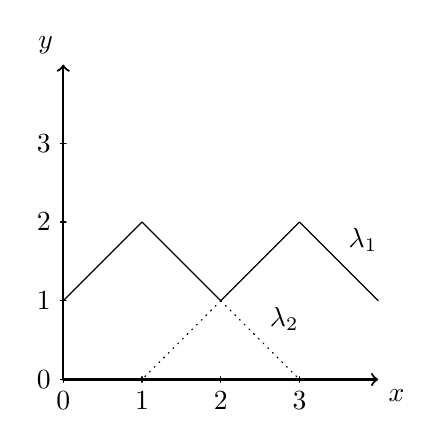
\begin{tikzpicture}[line cap=round, line join=round, x=1cm, y=1cm]
            
            \draw[thick,->] (0,0) -- (4,0) node[anchor=north west] {$x$};
            \draw[thick,->] (0,0) -- (0,4) node[anchor=south east] {$y$};

            \draw (0 cm,1pt) -- (0 cm,-1pt) node[anchor=north] {0};
            \draw (1 cm,1pt) -- (1 cm,-1pt) node[anchor=north] {1};
            \draw (2 cm,1pt) -- (2 cm,-1pt) node[anchor=north] {2};
            \draw (3 cm,1pt) -- (3 cm,-1pt) node[anchor=north] {3};

            \draw (1pt,0 cm) -- (-1pt,0 cm) node[anchor=east] {0};
            \draw (1pt,1 cm) -- (-1pt,1 cm) node[anchor=east] {1};
            \draw (1pt,2 cm) -- (-1pt,2 cm) node[anchor=east] {2};
            \draw (1pt,3 cm) -- (-1pt,3 cm) node[anchor=east] {3};

            \draw (0, 1) -- (1, 2) -- (2, 1);
            \draw[dotted] (2, 1) -- (3,0);

            \draw (2, 1) -- (3, 2) -- (4, 1);
            \draw[dotted] (2, 1) -- (1,0);

            \draw (2.5, 0.5) node[above right] {$\lambda_2$};
            \draw (3.5, 1.5) node[above right] {$\lambda_1$};
            
        \end{tikzpicture}
        \caption{}
        \label{fig:means-b}
    \end{subfigure}
    \begin{subfigure}[b]{0.45\linewidth}
        \centering
        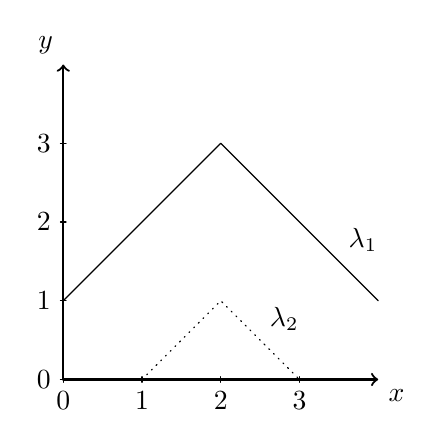
\begin{tikzpicture}[line cap=round, line join=round, x=1cm, y=1cm]
            
            \draw[thick,->] (0,0) -- (4,0) node[anchor=north west] {$x$};
            \draw[thick,->] (0,0) -- (0,4) node[anchor=south east] {$y$};

            \draw (0 cm,1pt) -- (0 cm,-1pt) node[anchor=north] {0};
            \draw (1 cm,1pt) -- (1 cm,-1pt) node[anchor=north] {1};
            \draw (2 cm,1pt) -- (2 cm,-1pt) node[anchor=north] {2};
            \draw (3 cm,1pt) -- (3 cm,-1pt) node[anchor=north] {3};

            \draw (1pt,0 cm) -- (-1pt,0 cm) node[anchor=east] {0};
            \draw (1pt,1 cm) -- (-1pt,1 cm) node[anchor=east] {1};
            \draw (1pt,2 cm) -- (-1pt,2 cm) node[anchor=east] {2};
            \draw (1pt,3 cm) -- (-1pt,3 cm) node[anchor=east] {3};

            \draw (0, 1) -- (2, 3) -- (4, 1);
            \draw[dotted] (1,0) -- (2, 1) -- (3,0);

            \draw (2.5, 0.5) node[above right] {$\lambda_2$};
            \draw (3.5, 1.5) node[above right] {$\lambda_1$};
            
        \end{tikzpicture}
        \caption{}
        \label{fig:means-c}
    \end{subfigure}
    \begin{subfigure}[b]{0.45\linewidth}
        \centering
        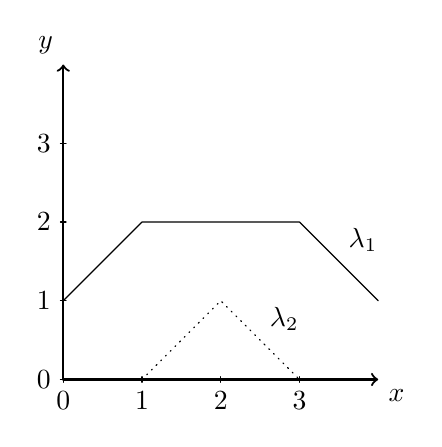
\begin{tikzpicture}[line cap=round, line join=round, x=1cm, y=1cm]
            
            \draw[thick,->] (0,0) -- (4,0) node[anchor=north west] {$x$};
            \draw[thick,->] (0,0) -- (0,4) node[anchor=south east] {$y$};

            \draw (0 cm,1pt) -- (0 cm,-1pt) node[anchor=north] {0};
            \draw (1 cm,1pt) -- (1 cm,-1pt) node[anchor=north] {1};
            \draw (2 cm,1pt) -- (2 cm,-1pt) node[anchor=north] {2};
            \draw (3 cm,1pt) -- (3 cm,-1pt) node[anchor=north] {3};

            \draw (1pt,0 cm) -- (-1pt,0 cm) node[anchor=east] {0};
            \draw (1pt,1 cm) -- (-1pt,1 cm) node[anchor=east] {1};
            \draw (1pt,2 cm) -- (-1pt,2 cm) node[anchor=east] {2};
            \draw (1pt,3 cm) -- (-1pt,3 cm) node[anchor=east] {3};

            \draw (0, 1) -- (1,2) -- (3,2) -- (4, 1);
            \draw[dotted] (1,0) -- (2, 1) -- (3,0);

            \draw (2.5, 0.5) node[above right] {$\lambda_2$};
            \draw (3.5, 1.5) node[above right] {$\lambda_1$};
            
        \end{tikzpicture}
        \caption{}
        \label{fig:means-d}
    \end{subfigure}
    \caption[Means from persistence landscapes]{The rescaled persistence diagrams of \ref{fig:means-a}, $\{(1, 2), (3, 2)\}$ and $\{(2, 1), (2, 3)\}$ have two (Fréchet) means: $\{(1.5, 2.5), (2.5, 1.5)\}$ and $\{(1.5, 1.5), (2.5, 2.5)\}$. In contrast, their corresponding persistence landscapes \ref{fig:means-b} and \ref{fig:means-c} have a unique mean \ref{fig:means-d}.}
    \label{fig:landscape-means}
\end{figure}